
%\documentclass{article}
\documentclass[tikz]{standalone}

\usepackage{pgf}
\usepackage{tikz}
\usetikzlibrary{arrows,automata,positioning}
%\usepackage[latin1]{inputenc}
\usepackage{verbatim}
\usepackage{graphicx}

\usetikzlibrary{shapes,arrows,positioning}
\tikzset{
  font={\fontsize{9pt}{11}\selectfont}
}

\definecolor{colorR}{RGB}{228,26,28}    % RED
\definecolor{colorB}{RGB}{55,126,184}   % BLUE
\definecolor{colorG}{RGB}{77,175,74}    % GREEN
\definecolor{colorP}{RGB}{152,78,163}   % PURPLE
\definecolor{colorO}{RGB}{255,127,0}    % ORANGE
\definecolor{colorY}{RGB}{255,255,51}   % YELLOW
\definecolor{colorBn}{RGB}{166,86,40}   % BROWN
\definecolor{colorPk}{RGB}{247,129,191} % PINK
\definecolor{colorGy}{RGB}{153,153,153} % GRAY

\begin{document}

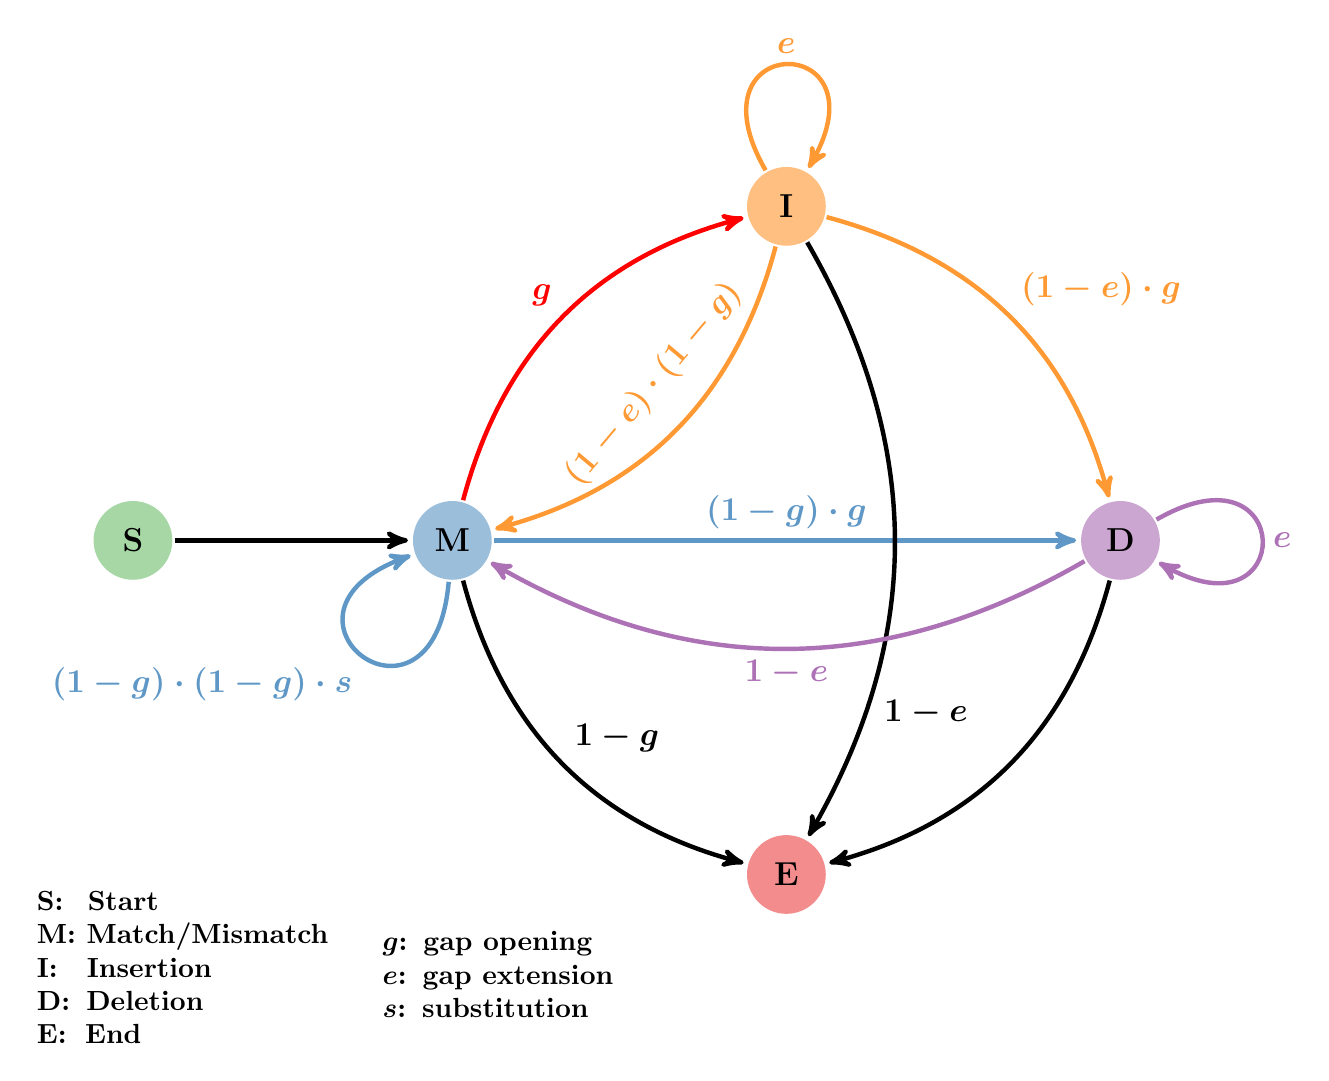
\begin{tikzpicture}[->,>=stealth',shorten >=1pt,auto,node distance=6cm,ultra thick]
  \tikzstyle{every node}=[font=\large]

  \node[circle,fill=colorG!50,minimum size=1cm]  (S)					  {\textbf{S}};
  \node[circle,fill=colorB!50,minimum size=1cm]	 (M) [right=30mm of S]  {\textbf{M}};
  \node[circle,fill=colorO!50,minimum size=1cm]  (I) [above right of=M] {\textbf{I}};
  \node[circle,fill=colorR!50,minimum size=1cm]  (E) [below right of=M] {\textbf{E}};
  \node[circle,fill=colorP!50,minimum size=1cm]  (D) [below right of=I] {\textbf{D}};

  \path (S) edge 			  node {}	(M)
  		(M) edge [colorB!80,out=265,in=200,looseness=10]  node [midway,font=\boldmath\large] {$(1-g)\cdot(1-g)\cdot s$} (M)
  			edge [red,bend left]  node [font=\boldmath\large] {$g$} (I)
            edge [colorB!80]        node [font=\boldmath\large] {$(1-g)\cdot g$} (D)
            edge [bend right] node [font=\boldmath\large] {$1-g$}	(E)
        (I) edge [colorO!80,out=120,in=60,looseness=10] node [font=\boldmath\large] {$e$} (I)
            edge [colorO!80,bend left]  node [rotate=50, above=1em, font=\boldmath\large] {$(1-e)\cdot (1-g)$} (M)
            edge [colorO!80,bend left]  node [font=\boldmath\large] {$(1-e) \cdot g $} (D)
            edge [bend left] node [near end, font=\boldmath\large] {$1-e$} (E)
        (D) edge [colorP!80,out=30,in=330,looseness=10] node [font=\boldmath\large] {$e$} (D)
        	edge [colorP!80,bend left]  node [font=\boldmath\large] {$1-e$} (M)
        	edge [bend left]  node {}	(E);

  \node[text width=4cm, below left=-3mm and 50mm of E, font=\bfseries] (T1) {S: \hspace{0.4mm} Start\\
  M: Match/Mismatch\\
  I: \hspace{1mm} Insertion\\
  D: \hspace{0.7mm}Deletion\\
  E: \hspace{1mm}End};

  \node[text width=5cm, right=1mm of T1, font=\bfseries\boldmath] (T2) {\\ $g$: gap opening\\ $e$: gap extension\\ $s$: substitution};

\end{tikzpicture}


\end{document}
